\begin{problem}
Найти распределение $\mu $. Вычислить $\Expect \mu$ и $\Variance\mu$.
Построить график функции распределения $F_\mu(m).$
\end{problem}

\begin{proof}
    $\mu= \sympy{mu}$

    \begin{sympycode}
m = symbols("m")
mu_eq = mu.subs("eta", y).subs("xi", x) - m
\end{sympycode}

    Изобразим область D и прямую  $\sympy{mu_eq}$:
    \begin{figure}[h!]
        \centering
        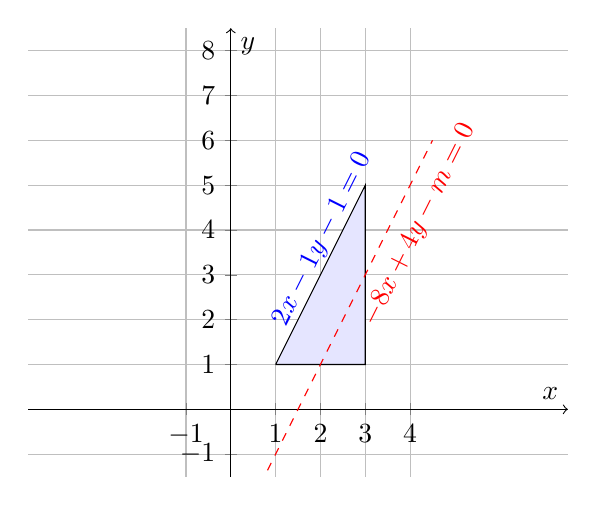
\begin{tikzpicture}
            \begin{axis}[
                    xlabel=$x$,
                    ylabel=$y$,
                    xmin=-1.5, xmax=4.5,
                    ymin=-1.5, ymax=8.5,
                    axis lines=middle,
                    axis line style={->},
                    % ticks=none,
                    clip=true,
                    xtick={-1,0,1,2,3,4},
                    ytick={-1,0,1,2,3,4,5,6,7,8},
                    axis equal,
                    grid=both,
                ]
                \addplot[fill=blue!10] coordinates {(1,1) (3, 5) (3, 1) (1,1)};
                \addplot[domain=-1.5:4.5, red, dashed] {2*x - 3};
                \node[blue, right, rotate=63.435] at (axis cs: 1, 1.7) {$2x-1y-1=0$};
                \node[red, right, rotate=63.435] at (axis cs: 3, 1.7) {$-8x + 4y - m = 0$};
            \end{axis}
        \end{tikzpicture}
        \caption{Область $D$ и прямая $-8x + 4y - m = 0$}
        \label{fig:D_m}
    \end{figure}

\begin{sympycode}
# mu_eq = mu_eq.subs("m",4)
y_m = solve(mu_eq, y)[0]
x_m = solve(mu_eq, x)[0]
x1_m = x_m.subs(y, y1)
y2_m = y_m.subs(x, x2)
x_interval_m = Interval(x1_m, x2)
y_interval_by_x_m = Interval(y1, y_m)
m1 = solve(mu_eq, m)[0].subs(y, y_interval_by_x.start).subs(x, x_interval.end)
m2 = solve(mu_eq, m)[0].subs(y, y_interval_by_x.end).subs(x, x_interval.end)
m_interval = Interval(m1, m2)
F_mu = integrate(p_xi_eta,  (y, y_interval_by_x_m.start, y_interval_by_x_m.end), 
                            (x, x_interval_m.start, x_interval_m.end)).simplify()
    \end{sympycode}
        
    По определению функция распределения случайной величины $\mu$:


    \[ \begin{aligned}
        F_\mu(m)
         & = \Prob(\mu \leq m) = \Prob(\sympy{mu} \leq m)                                                                                  \\
         & = \int\limits_{-\infty}^{+\infty} \int\limits_{-\infty}^{+\infty} p_{\xi, \eta}(x, y) \cdot \ind{\sympy{mu} \leq m} \, dx \, dy
        = \int\limits_{\sympy{x_interval_m.start}}^{\sympy{x_interval_m.end}} \, dx
        \int\limits_{\sympy{y_interval_by_x_m.start}}^{\sympy{y_interval_by_x_m.end}} \sympy{p_xi_eta} \, dy
         & = \sympy{F_mu}.
    \end{aligned}
\]

\begin{sympycode}
F_mu1 = Piecewise((0, m <= m_interval.start),
                    (F_mu, m <= m_interval.end),
                    (1, True))
\end{sympycode}

В точке  $(x;y) = (3; 1)$ прямая $-8x + 4y - m = 0$ пересекает область $D$ при единственном значении $m = \sympy{m_interval.start}$.



    \[
        F_\mu(m) \sympy{F_mu1}
    \]



    \begin{figure}[h!]
        \centering
        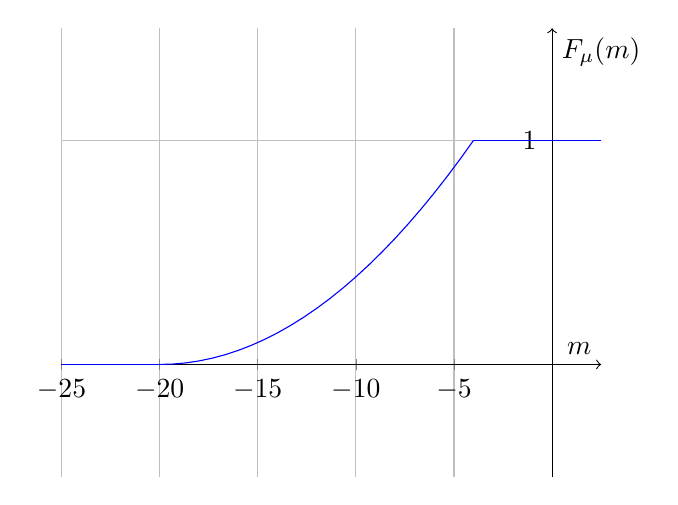
\begin{tikzpicture}
            \begin{axis}[
                    xlabel=$m$,
                    ylabel=$F_\mu(m)$,
                    xmin=-25, xmax=2.5,
                    ymin=-0.5, ymax=1.5,
                    axis lines=middle,
                    axis line style={->},
                    % ticks=none,
                    clip=true,
                    % xtick={-4,-3,-2,-1,0,1,2},
                    ytick={0,1},
                    grid=both,
                ]
                \addplot[domain=-25:-20, blue, solid] {0};
                \addplot[domain=-20:-4, blue, solid] {x^2/256 + 5*x/32 + 25/16};
                \addplot[domain=-4:6.5, blue, solid] {1};
            \end{axis}
        \end{tikzpicture}
        \caption{График функции распределения $F_\mu(m)$}
        \label{fig:F_mu}
    \end{figure}

    \begin{sympycode}
p_mu = diff(F_mu, m)
Expect_mu = integrate(m * p_mu, (m, m_interval.start, m_interval.end))
Expect_mu = Expect_mu.simplify()
p_mu1 = Piecewise((p_mu, And(m <= m_interval.end, m>=m_interval.end)), (0, True))
Expect_mu_quare = integrate(m ** 2 * p_mu, (m, m_interval.start, m_interval.end))
Variance_mu = Expect_mu_quare - Expect_mu ** 2
\end{sympycode}
    Найдём плотность распределения случайной величины $\mu$:
    \[
        p_\mu(m) = \frac{d F_\mu(m)}{d m} = \sympy{p_mu1}
    \]

    Найдём математическое ожидание и дисперсию случайной величины $\mu$:
    \[
        \begin{aligned}
            \Expect \mu
             & = \int\limits_{-\infty}^{+\infty} m \cdot p_\mu(m) \, dm
            = \int\limits_{\sympy{m_interval.start}}^{\sympy{m_interval.end}} m \cdot \left(\sympy{p_mu}\right) \, dm
            = \sympy{Expect_mu}
            \\
            \Variance \mu
             & = \Expect \mu^2 - (\Expect \mu)^2
            = \int\limits_{-\infty}^{+\infty} m^2 \cdot p_\mu(m) \, dm - (\Expect \mu)^2
            = \int\limits_{\sympy{m_interval.start}}^{\sympy{m_interval.end}} m^2 \cdot \left(\sympy{p_mu}\right) \, dm
            -  \left( \sympy{Expect_mu} \right)^2
            = \sympy{Expect_mu_quare} - \left( \sympy{Expect_mu} \right)^2
            = \sympy{Variance_mu}
        \end{aligned}
    \]
\end{proof}